% Preamble
\documentclass[a4paper, 12pt]{article}
\usepackage[margin=1in]{geometry} % Set margin
\usepackage{pdfpages} % Insert pdf pages
\usepackage{amssymb,amsmath,amsthm, amsfonts} % Math libraries

% Custom commands
\newcommand{\sub}[1]{\subsection{\underline{#1}}}
\newcommand{\subsub}[1]{\subsubsection{\underline{#1}}}
\newcommand{\R}{\ensuremath{\mathbb{R}}}
\newcommand{\F}{\ensuremath{\mathbb{F}}}
\newcommand{\N}{\ensuremath{\mathbb{N}}}
\newcommand{\Onef}{\ensuremath{1_{\F}}}
\newcommand{\Zerof}{\ensuremath{0_{\F}}}
\newcommand{\eqbcuz}[1]{\text{~$\stackrel{(#1)}{=}$~}}
\newcommand{\eq}[1]{\begin{align*}#1\end{align*}}
\newcommand{\eqn}[1]{\begin{align}#1\end{align}}
\newcommand{\set}[1]{\big{\{} #1 \big{\}}}
\newcommand{\bigset}[1]{\bigg{\{} #1 \bigg{\}}}
\renewcommand{\qed}{\hfill\(\qedsymbol\)}
\newtheorem{lemma}{Lemma}

% Begin Document %
\begin{document}

% Title Page
\begin{titlepage}
    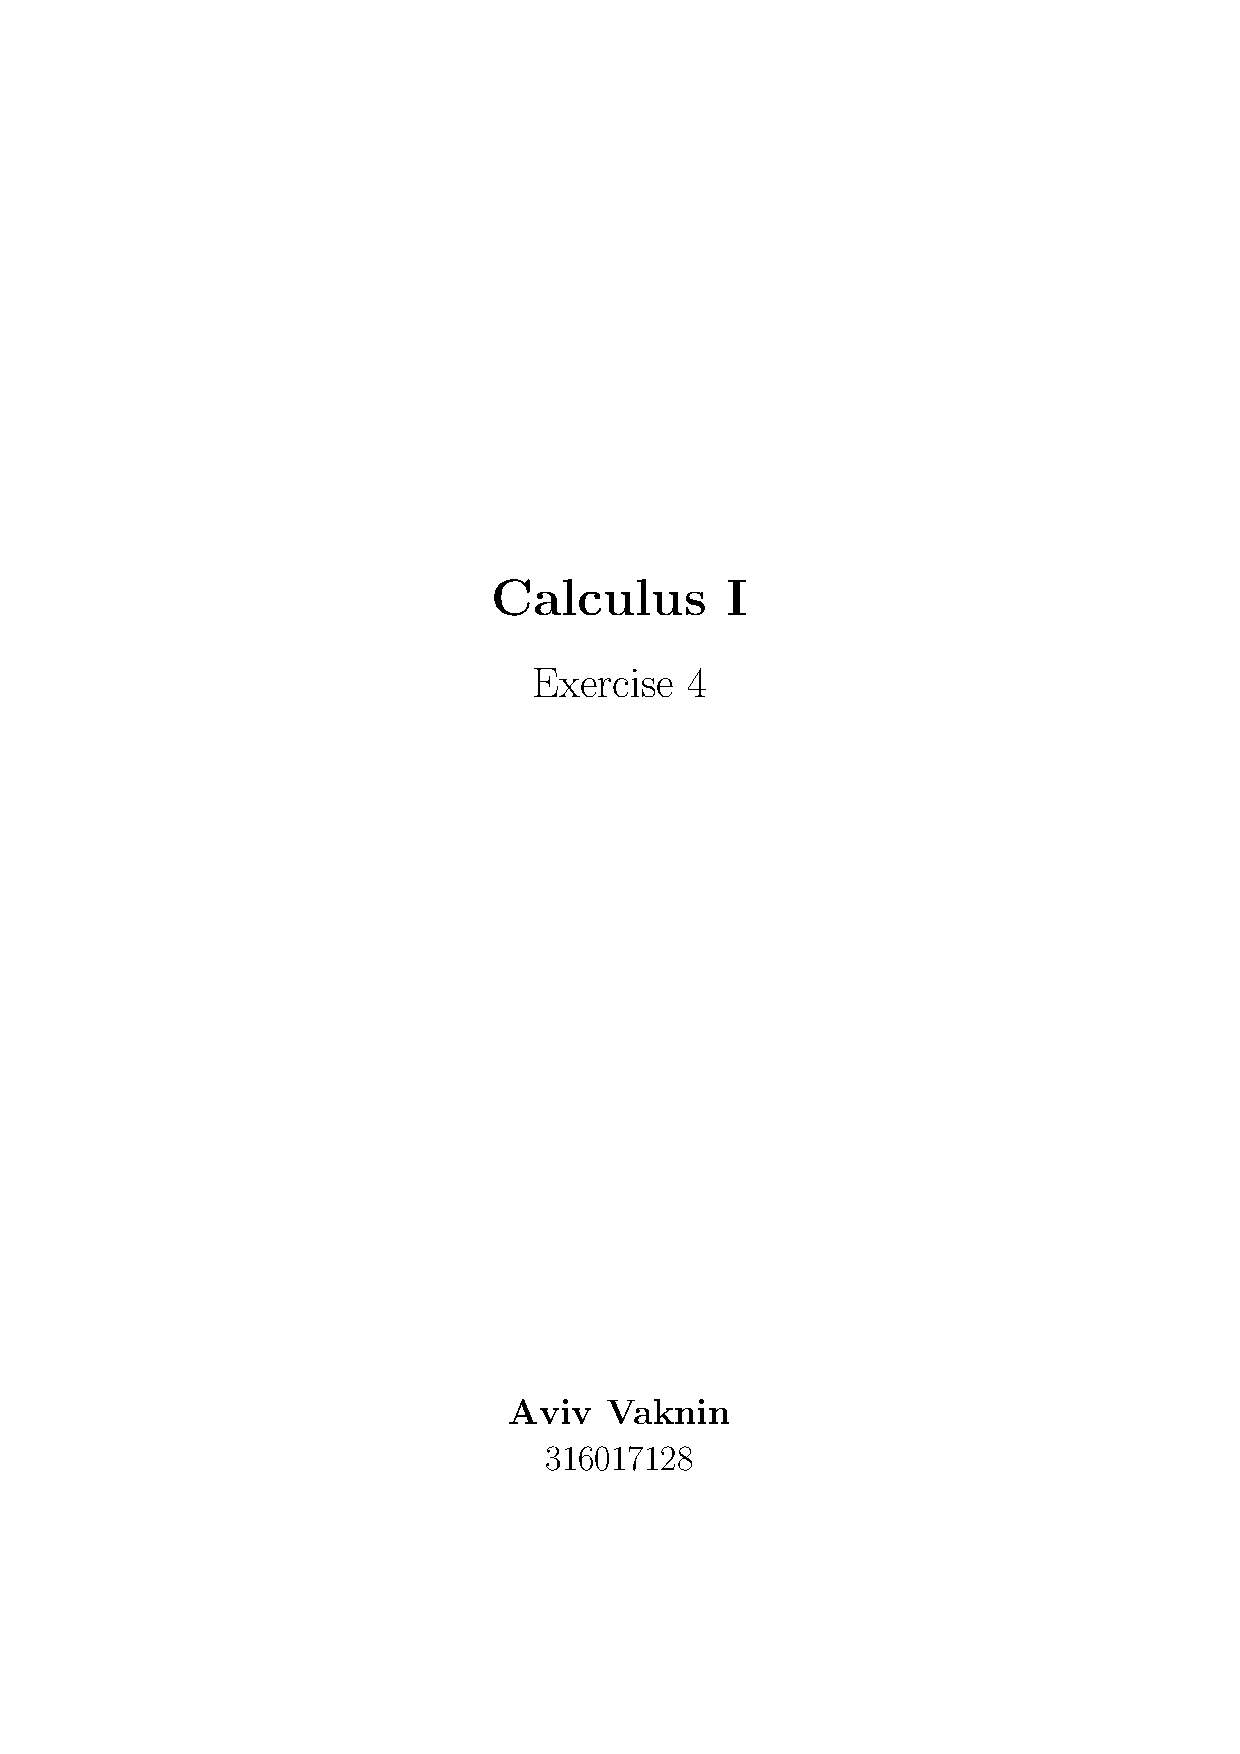
\includepdf{title.pdf}
\end{titlepage}

%1
\section{Prove \eq{
    \sup(\set{|x-y|~\big{|}~x,y\in{A}})=\sup{A}-\inf{A}
}}
First, let: \eq{D=\set{|x-y|~\big{|}~x,y\in{A}}}
We can see that \textit{D} consists of all of the distances in \textit{A}.\\
As we're searching for the supremum of this set, we're looking for the greatest \textit{x} and smallest \textit{y} values, that is:
\eq{
    x\in{A},~~x&=\max(A)\\
    y\in{A},~~y&=\min(A)\\
    |x-y|&=\max(D)
}
Possible candidates for min and max of a set, are the \textit{sup} and \textit{inf} of a set.\\
It is given that $A\in\R$, $A\neq\varnothing$ and that \textit{A} is bounded.\\
Therefore, according to the suprema and infima theorems, we can conclude that \textit{A} has a supremum and an infimum, such that:
\eq{
    &\sup(A)=s\\
    &\inf(A)=i
}
The only issue right now, is that \textit{s} and \textit{i} are unnecessarily part of \textit{A}.\\
Therefore, if we deduct or add some arbitrary $\frac{\epsilon}{2}>0$ from them, because of the definition of the supremum and infimum, they must be part of \textit{A}.
\eq{
    &x=\max(A)=s-\frac{\epsilon}{2}\\
    &y=\min(A)=i+\frac{\epsilon}{2}\\
    &x,y\in{A}
}
And therefore:
\eq{
    |x-y|=|s-\frac{\epsilon}{2}-(i+\frac{\epsilon}{2})|=|s-i-\epsilon|
}
According to definition, the supremum of a non-empty set must be greater than its infimum, therefore:
\eq{
    s&>i\\
    s&>i+\epsilon\\
    s-i-\epsilon&>0\\
    |s-i-\epsilon|&=s-i-\epsilon
}
Computing the supremum of D, we'll receive:
\eq{
    &\sup(D)=\sup(\{s-i-\epsilon\})=(s-i-\epsilon)+\epsilon=s-i\\
    &\sup(D)=\sup(A)-\inf(A)=s-i
}
\qed

%2
\section{Are the following subsets bounded from above or below? if yes, calculate the infimum/supremum, and decide whether there exist a min/max and compute them.}
\sub{}
\eq{
    A=\bigg{\{}
        \frac{3n+2}{n+5}~\bigg{|}~n\in\N
    \bigg{\}}
}
In order to work with this set, it'll be easier to first factor the term:
\eq{
    \frac{3n+2}{n+5}=\frac{3n+15}{n+5}-\frac{13}{n+5}=3-\frac{13}{n+5}
}
\subsub{lower-bound, infimum and minimum}
Now, it is easier to see that the term is smallest when $n=1$:
\eq{
    3-\frac{13}{6}=\frac{5}{6}
}
Thus, we can conclude that $i=\frac{5}{6}$ is the lower-bound, infimum and minimum of \textit{A}.
That is because $i\in{A}$, no other member of A is smaller than \textit{i}, and because it is the greatest lower-bound,
as if we'd increase its value, it would no longer be a lower-bound.
\subsub{higher-bound, supremum and maximum}
We can notice that as \textit{n} increases, the term $\frac{13}{n+5}$ is getting smaller and smaller, making the entire term closer and closer to 3.\\
Therefore, \textit{A} is bounded from above by 3, and it is its supremum as well.\\
However, \textit{A} does not have a maximum, because as n increases, the values get bigger.
\setcounter{subsection}{2}
\sub{}
\eq{
    C=\bigset{
        x\in\R~\big{|}~|x^2-4|\leq{5}
    }        
}
First, it is important to understand that $|x^2-4|\leq{5}$ implies that the only members that are in C fulfill:
\eq{
    \forall{c}\in{C}~-3\leq{c}\leq{3}
}
Therefore, it is quite easy to show that the lower-bound, infimum and minimum are -3,\\
while the higher-bound, supremum and maximum are 3.\\
That is because they exist in the set, no other member in the set is smaller or greater than them, and if we increase or decrease them, they will no longer be part of \textit{C}.
\qed\pagebreak

% 3
\section{Prove \eq{sup(A)=\sqrt{2}}}

% End
\end{document}